\documentclass[10pt]{book}

%These tell TeX which packages to use.
\usepackage{array,epsfig}
\usepackage{amsmath}
\usepackage{amsfonts}
\usepackage{amssymb}
\usepackage{amsxtra}
\usepackage{amsthm}
\usepackage{mathrsfs}
\usepackage{color}
\usepackage{enumitem}

\usepackage{pgfplots}
\pgfplotsset{compat=1.6}

\pgfplotsset{soldot/.style={color=black,only marks,mark=*}} \pgfplotsset{holdot/.style={color=black,fill=white,only marks,mark=*}}

%Here I define some theorem styles and shortcut commands for symbols I use often
\theoremstyle{definition}
\newtheorem{defn}{Definition}
\newtheorem{thm}{Theorem}
\newtheorem{cor}{Corollary}
\newtheorem*{rmk}{Remark}
\newtheorem{lem}{Lemma}
\newtheorem*{joke}{Joke}
\newtheorem{ex}{Example}
\newtheorem*{soln}{Solution}
\newtheorem{prop}{Proposition}

\newcommand{\lra}{\longrightarrow}
\newcommand{\ra}{\rightarrow}
\newcommand{\surj}{\twoheadrightarrow}
\newcommand{\graph}{\mathrm{graph}}
\newcommand{\bb}[1]{\mathbb{#1}}
\newcommand{\Z}{\bb{Z}}
\newcommand{\Q}{\bb{Q}}
\newcommand{\R}{\bb{R}}
\newcommand{\C}{\bb{C}}
\newcommand{\N}{\bb{N}}
\newcommand{\M}{\mathbf{M}}
\newcommand{\m}{\mathbf{m}}
\newcommand{\MM}{\mathscr{M}}
\newcommand{\HH}{\mathscr{H}}
\newcommand{\Om}{\Omega}
\newcommand{\Ho}{\in\HH(\Om)}
\newcommand{\bd}{\partial}
\newcommand{\del}{\partial}
\newcommand{\bardel}{\overline\partial}
\newcommand{\textdf}[1]{\textbf{\textsf{#1}}\index{#1}}
\newcommand{\img}{\mathrm{img}}
\newcommand{\ip}[2]{\left\langle{#1},{#2}\right\rangle}
\newcommand{\inter}[1]{\mathrm{int}{#1}}
\newcommand{\exter}[1]{\mathrm{ext}{#1}}
\newcommand{\cl}[1]{\mathrm{cl}{#1}}
\newcommand{\ds}{\displaystyle}
\newcommand{\vol}{\mathrm{vol}}
\newcommand{\cnt}{\mathrm{ct}}
\newcommand{\osc}{\mathrm{osc}}
\newcommand{\LL}{\mathbf{L}}
\newcommand{\UU}{\mathbf{U}}
\newcommand{\support}{\mathrm{support}}
\newcommand{\AND}{\;\wedge\;}
\newcommand{\OR}{\;\vee\;}
\newcommand{\Oset}{\varnothing}
\newcommand{\st}{\ni}
\newcommand{\wh}{\widehat}
%Pagination stuff.
\setlength{\topmargin}{-0.75in}
\setlength{\oddsidemargin}{0in}
\setlength{\evensidemargin}{0in}
\setlength{\textheight}{9.in}
\setlength{\textwidth}{6.5in}
\pagestyle{empty}
\begin{document}
\begin{flushleft}
Name:\underline{\hspace{13cm}}Date:\underline{\hspace{2cm}}
\end{flushleft}
\begin{center}
{\Large Math 1041-007 \hspace{0.5cm} Quiz \#1}
\end{center}
\vspace{0.2 cm}
\subsection*{Problem 1} A rock is thrown into the air with a velocity of $60$ ft/s, its height in feet at $t$ seconds is given by $h=60t-16t^2$.
\begin{itemize}
    \item[(a)] Find the height of the rock after 2 seconds.
    
    \item[(b)] Find the average velocity for the time period beginning when $t=2$ and lasting 1 second.
\end{itemize}
\vspace{2.5in}
\subsection*{Problem 2} \underline{Sketch} the graph of the function and use it to determine the values of $a$ for which $\displaystyle\lim_{x\rightarrow a}f(x)$ exists. Use your sketch to find the indicated limits! If a limit does not exist write DNE. :)
\[
f(x)=\begin{cases}
-(x+1) & x< -1\\
1-x^2 & -1\leq x<1\\
x & x\geq 1
\end{cases}
\]
\begin{itemize}
    \item[(a)]$\displaystyle\lim_{x\rightarrow 0}f(x)$
    \item[(b)]$\displaystyle\lim_{x\rightarrow 1^-}f(x)$
    \item[(c)]$\displaystyle\lim_{x\rightarrow 1^+}f(x)$
    \item[(d)]$\displaystyle\lim_{x\rightarrow 1}f(x)$
    \item[(e)]$\displaystyle\lim_{x\rightarrow -1}f(x)$
\end{itemize}
\clearpage
\subsection*{Problem $\pi$} For the function $f(x)$ whose graph is shown below state each of the following limits. If a limit does not exist, write DNE. :)
\begin{figure}[h]
    \centering
    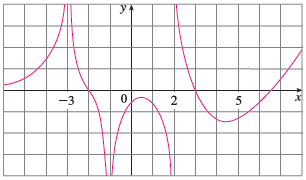
\includegraphics{fig1.png}
\end{figure}
\begin{itemize}
    \item[(a)] $\displaystyle\lim_{x\rightarrow -2}f(x)$
    \item[(b)] $\displaystyle\lim_{x\rightarrow 2^+}f(x)$
    \item[(c)] $\displaystyle\lim_{x\rightarrow 2^-}f(x)$
    \item[(d)] $\displaystyle\lim_{x\rightarrow 2}f(x)$
    \item[(e)] $\displaystyle\lim_{x\rightarrow -3}f(x)$
    \item[(f)] Write the equation(s) of the vertical asymptotes.
\end{itemize}
\subsection*{Problem 4} The graphs of $f$ and $g$ are given. Use them to evaluate each limit if it exists. If the limit does not exist \underline{explain why!!}
\begin{figure}[h]
    \centering
    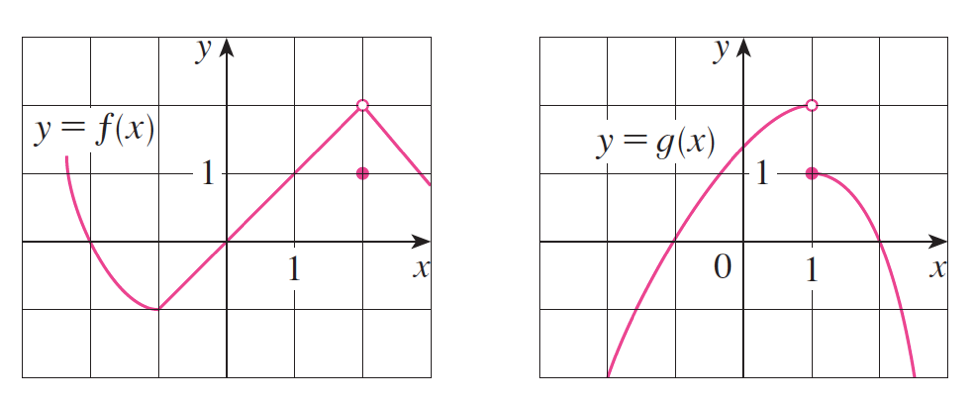
\includegraphics[scale=0.65]{fandg.png}
\end{figure}
\begin{itemize}
    \item[(a)] $\displaystyle\lim_{x\rightarrow 2^+}[2f(x)+g(x)]$ \vspace{3mm}
    \item[(b)] $\displaystyle\lim_{x\rightarrow 1}[f(x)-3g(x)]$\vspace{3mm}
    \item[(c)] $\displaystyle\lim_{x\rightarrow 2}\frac{f(x)}{g(x)+1}$\vspace{3mm}
    \item[(d)] $\displaystyle\lim_{x\rightarrow -1}2f(x)g(x)$ 
\end{itemize}
\end{document}
